\documentclass[12pt,a4paper]{article}
\usepackage[top=2.5cm,bottom=2.5cm,left=2.5cm,right=2.5cm,headheight=15pt]{geometry}
\usepackage{amsmath,amssymb}
\usepackage{tikz}
\usetikzlibrary{shapes,arrows,arrows.meta,positioning,calc,backgrounds,fit,matrix}
\usepackage{booktabs,array,longtable,tabularx,multirow}
\usepackage{xcolor}
\usepackage{enumitem}
\usepackage{fancyhdr}
\usepackage{titlesec}
\usepackage{mdframed}
\usepackage{tcolorbox}
\tcbuselibrary{skins,breakable}
\usepackage{hyperref}

%% ---- Colors ----
\definecolor{folblue}{RGB}{0,82,165}
\definecolor{lightblue}{RGB}{220,235,255}
\definecolor{darkorange}{RGB}{180,70,0}
\definecolor{lightorange}{RGB}{255,235,210}
\definecolor{darkgreen}{RGB}{20,110,20}
\definecolor{lightgreen}{RGB}{200,240,205}
\definecolor{darkred}{RGB}{150,20,20}
\definecolor{lightred}{RGB}{255,210,210}
\definecolor{lightgray}{RGB}{242,242,242}

%% ---- tcolorbox styles ----
\newtcolorbox{qbox}[2][]{enhanced,breakable,
  colback=lightorange,colframe=darkorange,arc=4pt,
  title={\textbf{#2}},fonttitle=\bfseries\color{white},
  attach boxed title to top left={yshift=-2mm,xshift=4mm},
  boxed title style={colback=darkorange,arc=3pt},#1}

\newtcolorbox{solbox}[2][]{enhanced,breakable,
  colback=lightblue,colframe=folblue,arc=4pt,
  title={\textbf{#2}},fonttitle=\bfseries\color{white},
  attach boxed title to top left={yshift=-2mm,xshift=4mm},
  boxed title style={colback=folblue,arc=3pt},#1}

\newtcolorbox{keybox}[2][]{enhanced,breakable,
  colback=lightgreen,colframe=darkgreen,arc=4pt,
  title={\textbf{#2}},fonttitle=\bfseries\color{white},
  attach boxed title to top left={yshift=-2mm,xshift=4mm},
  boxed title style={colback=darkgreen,arc=3pt},#1}

\newtcolorbox{algobox}[2][]{enhanced,breakable,
  colback=lightgray,colframe=gray!60,arc=4pt,
  title={\textbf{#2}},fonttitle=\bfseries,
  attach boxed title to top left={yshift=-2mm,xshift=4mm},
  boxed title style={colback=gray!60,arc=3pt},#1}

\newtcolorbox{warnbox}[2][]{enhanced,breakable,
  colback=lightred,colframe=darkred,arc=4pt,
  title={\textbf{#2}},fonttitle=\bfseries\color{white},
  attach boxed title to top left={yshift=-2mm,xshift=4mm},
  boxed title style={colback=darkred,arc=3pt},#1}

%% ---- Page style ----
\pagestyle{fancy}\fancyhf{}
\lhead{\color{folblue}\textbf{DES / Feistel / S-box / Avalanche / 3-DES --- CSE 717 InfoSec}}
\rhead{\color{folblue}Exam: 17 Jun 2026}
\cfoot{--- \thepage\ ---}
\renewcommand{\headrulewidth}{0.4pt}

%% ---- Section style ----
\titleformat{\section}{\large\bfseries\color{folblue}}{}{0em}{}[\titlerule]
\titleformat{\subsection}{\normalsize\bfseries\color{darkorange}}{}{0em}{}

\begin{document}

\begin{center}
{\LARGE\bfseries\color{folblue} CSE 717 --- Information Security}\\[4pt]
{\large\bfseries Topic 13: DES / Feistel Structure / S-box / Avalanche Effect / 3-DES}\\[2pt]
{\large Complete Past Paper Solutions: 2020--2024}\\[6pt]
{\normalsize Source: general security knowledge (Stallings DES) --- NOT in any 2026 Lc material, but CONFIRMED EVERY YEAR}\\[2pt]
{\normalsize\color{darkred}\textbf{Every Topic-13 question 2020--2024 included. Zero omissions.}}
\end{center}

\tableofcontents
\newpage

%% ==========================================
\section*{Quick Reference --- The 6 Recurring Sub-Patterns (CHEAT SHEET)}
%% ==========================================

\begin{warnbox}{Not in any 2026 Lc material --- CONFIRMED GUARANTEED every year (5/5, 5--10 marks)}
None of Lc\#1--11 cover DES/Feistel/3-DES content. Everything below is standard textbook (Stallings) knowledge memorized as a cheat sheet --- ~45min investment for ~6--10 guaranteed marks.
\end{warnbox}

\begin{algobox}{1. Classical Feistel Cipher Structure}
\begin{enumerate}[noitemsep]
  \item Split the plaintext block into two equal halves: $L_0$ (left) and $R_0$ (right).
  \item For each round $i = 1, \dots, n$ (DES uses $n=16$):
  \[
  L_i = R_{i-1}, \qquad R_i = L_{i-1} \oplus F(R_{i-1}, K_i)
  \]
  where $F$ is the round (mangler) function and $K_i$ is the $i$-th round subkey.
  \item After the final round, the two halves are \textbf{combined} (and typically swapped back) to form the ciphertext block.
\end{enumerate}

\textbf{One-round diagram:}
\begin{center}
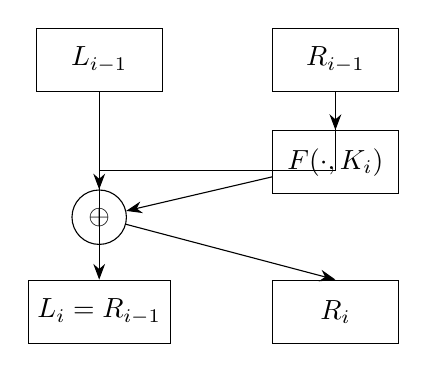
\begin{tikzpicture}[
  box/.style={draw, rectangle, minimum width=1.6cm, minimum height=0.8cm, align=center},
  circ/.style={draw, circle, minimum size=0.6cm},
  >={Stealth[length=2mm]}
]
  \node[box] (Lprev) at (0,2) {$L_{i-1}$};
  \node[box] (Rprev) at (3,2) {$R_{i-1}$};
  \node[box] (F) at (3,0.7) {$F(\cdot,K_i)$};
  \node[circ] (xor) at (0,0) {$\oplus$};
  \node[box] (Li) at (0,-1.2) {$L_i = R_{i-1}$};
  \node[box] (Ri) at (3,-1.2) {$R_i$};

  \draw[->] (Rprev) -- (F);
  \draw[->] (Rprev.south) -- ++(0,-1.0) -| (Li.north);
  \draw[->] (Lprev) -- (xor);
  \draw[->] (F) -- (xor);
  \draw[->] (xor) -- (Ri.north);
\end{tikzpicture}
\end{center}

\textbf{Key property:} the SAME algorithm performs both encryption and decryption --- decryption simply applies the subkeys $K_n, \dots, K_1$ in \textbf{reverse order}. This symmetry is the entire point of a Feistel network.
\end{algobox}

\begin{algobox}{2. DES Overview + IP / IP$^{-1}$ Permutations}
\begin{itemize}[noitemsep]
  \item \textbf{DES parameters:} 64-bit plaintext block, 56-bit effective key (64 bits incl.\ parity), \textbf{16 Feistel rounds}.
  \item \textbf{IP (Initial Permutation):} reorders the 64 input bits \emph{before} round 1. \textbf{Purpose:} purely a bit-level rearrangement for convenient loading into 1970s hardware registers --- has \textbf{no cryptographic significance} on its own.
  \item \textbf{IP$^{-1}$ (Final/Inverse Permutation):} applied \emph{after} round 16 to undo IP's bit-ordering and produce the 64-bit ciphertext:
  \[
  \text{Ciphertext} = IP^{-1}(R_{16} \,\|\, L_{16})
  \]
  (note the swap of the two halves before the final permutation --- this swap is what makes the SAME structure work for decryption).
\end{itemize}
\end{algobox}

\begin{algobox}{3. F-function (Round/Mangler Function) Components}
Input: $R_{i-1}$ (32 bits) and round subkey $K_i$ (48 bits). Steps:
\begin{enumerate}[noitemsep]
  \item \textbf{Expansion permutation $E$:} expands $R_{i-1}$ from 32 $\to$ 48 bits (some bits duplicated).
  \item \textbf{XOR with round key:} $E(R_{i-1}) \oplus K_i$ (48 bits).
  \item \textbf{S-box substitution:} the 48 bits are split into eight 6-bit groups, each passed through one of \textbf{8 S-boxes ($S_1$--$S_8$)}, each producing 4 bits $\to$ 32 bits total. \textbf{This is the only non-linear step} --- the core source of DES's security (confusion).
  \item \textbf{Permutation $P$:} a 32 $\to$ 32-bit straight permutation that shuffles the S-box outputs (diffusion).
\end{enumerate}
\[
F(R_{i-1},K_i) \;=\; P\Big(\, S\big(E(R_{i-1}) \oplus K_i\big) \,\Big)
\]
\textbf{Diagram (chain form):}
\[
R_{i-1} \xrightarrow{E\,(32\to48)} \boxed{\oplus K_i} \xrightarrow{} \boxed{S_1\dots S_8\,(48\to32)} \xrightarrow{P\,(32\to32)} F(R_{i-1},K_i)
\]
\end{algobox}

\begin{algobox}{4. S-box / S1-Box Lookup for Input 37 (recurs 2020 \& 2022)}
\textbf{Why S-boxes exist:} they are the \textbf{only non-linear component} of DES --- without them, DES would be a linear (and trivially breakable) cipher. S-boxes provide \textbf{confusion}.

\textbf{Lookup procedure (any 6-bit input $b_1b_2b_3b_4b_5b_6$):}
\begin{itemize}[noitemsep]
  \item \textbf{Row} = $b_1b_6$ (outer bits, as a 2-bit binary number, 0--3).
  \item \textbf{Column} = $b_2b_3b_4b_5$ (middle 4 bits, as a 4-bit binary number, 0--15).
  \item Look up $S_1[\text{row}][\text{column}]$ in the standard $S_1$ table.
\end{itemize}

\textbf{Worked example --- input 37:}
\begin{itemize}[noitemsep]
  \item $37 = 100101_2$ (6 bits).
  \item Row $= b_1b_6 = 11_2 = 3$. Column $= b_2b_3b_4b_5 = 0010_2 = 2$.
  \item $S_1$ table, row 3: \texttt{15 12 8 2 4 9 1 7 5 11 3 14 10 0 6 13} (columns 0--15).
  \item Column 2 $\to$ value $= \mathbf{8}$ (binary \texttt{1000}).
\end{itemize}
\[
\boxed{S_1(37) = 8}
\]
\end{algobox}

\begin{algobox}{5. Avalanche Effect + Two Families of DES Attacks (recurs EVERY year)}
\begin{itemize}[noitemsep]
  \item \textbf{Avalanche effect:} a small change in the input (even 1 bit of plaintext or key) should produce a \textbf{large, unpredictable change} in the output ciphertext (ideally $\sim$half the output bits flip). A strong avalanche effect makes statistical attacks hard.
  \item \textbf{Two families of attacks on DES:}
  \begin{enumerate}[noitemsep]
    \item \textbf{Differential cryptanalysis} (Biham \& Shamir) --- studies how differences in plaintext pairs propagate to differences in ciphertext pairs to recover key bits.
    \item \textbf{Linear cryptanalysis} (Matsui) --- finds linear approximations relating plaintext, ciphertext, and key bits that hold with probability $\neq 0.5$, exploited statistically over many samples.
  \end{enumerate}
\end{itemize}
\end{algobox}

\begin{algobox}{6. 3-DES (Triple DES) Block Diagram + Encryption Equation}
\textbf{Why 3-DES:} single DES's 56-bit key is too short (brute-forceable). 3-DES applies DES three times with (typically 2 or 3) different keys to extend effective key length, while staying \textbf{backward-compatible} with single DES.

\textbf{Encryption (EDE = Encrypt-Decrypt-Encrypt):}
\[
C = E_{K_3}\big(D_{K_2}(E_{K_1}(P))\big)
\]
\textbf{Decryption:}
\[
P = D_{K_1}\big(E_{K_2}(D_{K_3}(C))\big)
\]

\textbf{Block diagram (chain form):}
\[
P \xrightarrow{E_{K_1}} \boxed{\text{stage 1}} \xrightarrow{D_{K_2}} \boxed{\text{stage 2}} \xrightarrow{E_{K_3}} \boxed{\text{stage 3}} \rightarrow C
\]

\textbf{Why EDE (not EEE), and why a middle \emph{decrypt}:} if $K_1=K_2=K_3$, then $D_{K_2}(E_{K_1}(P)) = P$, so $C = E_{K_3}(P)$ --- i.e.\ 3-DES with all-equal keys collapses to \textbf{plain single DES}, giving \textbf{backward compatibility} with legacy single-DES systems. With 2 distinct keys ($K_1=K_3 \neq K_2$), effective key length $\approx 112$ bits; with 3 distinct keys, $\approx 168$ bits.
\end{algobox}

\begin{algobox}{Bonus: Finite Fields in Cryptography (one-liner, 2020 Q4(b))}
A \textbf{finite field $GF(2^n)$} is the set of all $n$-bit values with addition (bitwise XOR) and multiplication defined modulo an \textbf{irreducible polynomial} of degree $n$. This gives every non-zero element a multiplicative inverse --- the algebraic structure needed for \textbf{invertible} (hence decryptable) substitution operations. Used directly in AES ($GF(2^8)$, S-box \& MixColumns).
\end{algobox}

\newpage
%% ==========================================
\section{2024 --- Q6(d): Avalanche Effect + DES Attack Families (2 marks)}
%% ==========================================

\begin{qbox}{Question --- 2024 Q6(d)}
Explain the avalanche effect in the context of DES, and name the two families of attacks against DES. \hfill [2]
\end{qbox}

\begin{solbox}{Answer --- 2024 Q6(d)}
\begin{itemize}[noitemsep]
  \item \textbf{Avalanche effect:} a 1-bit change in the plaintext or key causes a large, unpredictable change in the ciphertext --- roughly half the output bits flip. This prevents an attacker from inferring small input changes from small output changes.
  \item \textbf{Two attack families:} \textbf{Differential cryptanalysis} (analyzes how input differences propagate to output differences) and \textbf{Linear cryptanalysis} (exploits linear approximations of the cipher that hold with non-trivial probability).
\end{itemize}
\textit{See Cheat Sheet \#5 for full definitions.}
\end{solbox}

\newpage
%% ==========================================
\section{2023 --- Q3(a,b): 3-DES + DES Equation, Avalanche (5 marks); Section B Q5(a): F-function (2.5 marks)}
%% ==========================================

\begin{qbox}{Question --- 2023 Q3}
\begin{enumerate}[label=(\alph*)]
  \item Draw the 3-DES block diagram and write the DES encryption equation. \hfill [3]
  \item Explain the avalanche effect and name the two families of attacks against DES. \hfill [2]
\end{enumerate}
\noindent\textbf{Section B Q5(a):} Describe the F-function (round function) used in DES. \hfill [2.5]
\end{qbox}

\subsection{Part (a): 3-DES Block Diagram + DES Encryption Equation}
\begin{solbox}{Answer --- 2023 Q3(a)}
\textbf{3-DES block diagram:} see Cheat Sheet \#6 --- $P \xrightarrow{E_{K_1}} \xrightarrow{D_{K_2}} \xrightarrow{E_{K_3}} C$.

\textbf{Single-DES encryption equation (per round):}
\[
L_i = R_{i-1}, \qquad R_i = L_{i-1} \oplus F(R_{i-1}, K_i), \qquad i = 1,\dots,16
\]
\[
\text{Ciphertext} = IP^{-1}(R_{16} \,\|\, L_{16})
\]
\end{solbox}

\subsection{Part (b): Avalanche Effect + Attack Families}
\begin{solbox}{Answer --- 2023 Q3(b)}
Same as 2024 Q6(d) above --- see Cheat Sheet \#5: \textbf{avalanche effect} (1-bit change $\to$ large unpredictable ciphertext change) + \textbf{differential} and \textbf{linear cryptanalysis}.
\end{solbox}

\subsection{Part Section B Q5(a): The F-function}
\begin{solbox}{Answer --- 2023 Section B Q5(a)}
The \textbf{F-function} (round/mangler function) takes $R_{i-1}$ (32 bits) and subkey $K_i$ (48 bits), and produces a 32-bit output via 4 stages:
\begin{enumerate}[noitemsep]
  \item \textbf{Expansion ($E$):} 32 $\to$ 48 bits (some bits duplicated).
  \item \textbf{XOR with $K_i$:} $E(R_{i-1}) \oplus K_i$.
  \item \textbf{S-box substitution:} eight 6-bit groups $\to$ eight S-boxes ($S_1$--$S_8$) $\to$ 32 bits (the only non-linear step --- confusion).
  \item \textbf{Permutation ($P$):} 32 $\to$ 32-bit shuffle (diffusion).
\end{enumerate}
\[
F(R_{i-1},K_i) = P\big(S(E(R_{i-1}) \oplus K_i)\big)
\]
\textit{See Cheat Sheet \#3 for the diagram.}
\end{solbox}

\newpage
%% ==========================================
\section{2022 --- Q4: S-box + 3-DES + F-function (8 marks)}
%% ==========================================

\begin{qbox}{Question --- 2022 Q4}
\begin{enumerate}[label=(\alph*)]
  \item Why is an S-box needed in DES? Given input value 37, find the corresponding $S_1$-box output. \hfill [2]
  \item Draw the 3-DES schematic and write the encryption equation. \hfill [3]
  \item Describe the components of the f-function (F-function) in DES. \hfill [3]
\end{enumerate}
\end{qbox}

\subsection{Part (a): Why S-box + S1-Box(37)}
\begin{solbox}{Answer --- 2022 Q4(a)}
\textbf{Why S-box:} the S-box is the \textbf{only non-linear element} in DES's round function --- it provides \textbf{confusion} (obscures the relationship between key and ciphertext). Without it, DES would be a purely linear transformation and trivially breakable by solving linear equations.

\textbf{$S_1$-box lookup for input 37:}
\begin{itemize}[noitemsep]
  \item $37 = 100101_2$. Row $=b_1b_6=11_2=3$, Column $=b_2b_3b_4b_5=0010_2=2$.
  \item $S_1$ row 3: \texttt{15 12 8 2 4 9 1 7 5 11 3 14 10 0 6 13} $\to$ column 2 $=\mathbf{8}$.
\end{itemize}
\[
\boxed{S_1(37) = 8}
\]
\end{solbox}

\subsection{Part (b): 3-DES Schematic + Encryption Equation}
\begin{solbox}{Answer --- 2022 Q4(b)}
See Cheat Sheet \#6:
\[
P \xrightarrow{E_{K_1}} \boxed{\text{stage 1}} \xrightarrow{D_{K_2}} \boxed{\text{stage 2}} \xrightarrow{E_{K_3}} \boxed{\text{stage 3}} \rightarrow C
\qquad
C = E_{K_3}\big(D_{K_2}(E_{K_1}(P))\big)
\]
With $K_1=K_2=K_3$, this collapses to single DES (backward compatibility). 2-key 3-DES ($K_1=K_3$) gives $\approx$112-bit effective security; 3-key gives $\approx$168-bit.
\end{solbox}

\subsection{Part (c): F-function Components}
\begin{solbox}{Answer --- 2022 Q4(c)}
Same 4-stage description as 2023 Section B Q5(a) above: \textbf{Expansion (32$\to$48)} $\to$ \textbf{XOR with $K_i$} $\to$ \textbf{S-box substitution (48$\to$32, 8 S-boxes)} $\to$ \textbf{Permutation $P$ (32$\to$32)}. See Cheat Sheet \#3 for the diagram.
\end{solbox}

\newpage
%% ==========================================
\section{2021 --- A4: IP$^{-1}$ Equation, 3-DES, Avalanche (9.5 marks)}
%% ==========================================

\begin{qbox}{Question --- 2021 A4}
\begin{enumerate}[label=(\roman*)]
  \item Explain the $IP^{-1}$ (inverse initial permutation) equation in DES. \hfill [part of 4.75]
  \item Draw the 3-DES block diagram and write its encryption equation. \hfill [2.75]
  \item Explain the avalanche effect and name the two families of attacks against DES. \hfill [2]
\end{enumerate}
\end{qbox}

\subsection{Part (i): IP$^{-1}$ Equation}
\begin{solbox}{Answer --- 2021 A4(i)}
After 16 Feistel rounds, the two 32-bit halves are \textbf{swapped} and the inverse initial permutation $IP^{-1}$ is applied to produce the final 64-bit ciphertext:
\[
\text{Ciphertext} = IP^{-1}(R_{16} \,\|\, L_{16})
\]
$IP^{-1}$ exactly \textbf{undoes} the bit-reordering performed by $IP$ at the start --- so $IP^{-1}(IP(X)) = X$. Neither $IP$ nor $IP^{-1}$ adds cryptographic strength; they exist only for hardware bit-ordering convenience (see Cheat Sheet \#2).
\end{solbox}

\subsection{Part (ii): 3-DES Block Diagram + Equation}
\begin{solbox}{Answer --- 2021 A4(ii)}
Identical to Cheat Sheet \#6: $P \xrightarrow{E_{K_1}} \xrightarrow{D_{K_2}} \xrightarrow{E_{K_3}} C$, with $C = E_{K_3}(D_{K_2}(E_{K_1}(P)))$.
\end{solbox}

\subsection{Part (iii): Avalanche Effect + Attack Families}
\begin{solbox}{Answer --- 2021 A4(iii)}
Same as Cheat Sheet \#5: \textbf{avalanche effect} + \textbf{differential cryptanalysis} \& \textbf{linear cryptanalysis}.
\end{solbox}

\newpage
%% ==========================================
\section{2020 --- Q4(a,b): IP/IP$^{-1}$, S1-Box(37), F-function, Finite Fields (9.5 marks); Section B Q5(a,b): 3-DES + Avalanche + Feistel (8.25 marks)}
%% ==========================================

\begin{qbox}{Question --- 2020 Q4 and Section B Q5}
\textbf{Q4.}
\begin{enumerate}[label=(\alph*)]
  \item Explain the purpose of $IP$ and $IP^{-1}$ in DES. Given input 37, find the $S_1$-box output. \hfill [2 + 2.75]
  \item Write the $IP^{-1}$ decryption equation. Briefly explain finite fields in cryptography. \hfill [part of total]
\end{enumerate}
\textbf{Section B Q5.}
\begin{enumerate}[label=(\alph*)]
  \item Draw the 3-DES block diagram and write its encryption equation (twice, 2.75$\times$2). \hfill [5.5]
  \item Explain the avalanche effect, the two families of attacks against DES, and the classical Feistel cipher structure. \hfill [2.75]
\end{enumerate}
\end{qbox}

\subsection{Part Q4(a): IP/IP$^{-1}$ Purpose + S1-Box(37)}
\begin{solbox}{Answer --- 2020 Q4(a)}
\textbf{Purpose of $IP$ / $IP^{-1}$:} $IP$ reorders the 64 input bits before round 1; $IP^{-1}$ undoes this reordering after round 16 (applied to $R_{16}\|L_{16}$) to produce the ciphertext. \textbf{Neither adds cryptographic strength} --- purely a hardware bit-loading convenience (see Cheat Sheet \#2).

\textbf{$S_1$-box(37):} same computation as Cheat Sheet \#4 $\to \boxed{S_1(37)=8}$.
\end{solbox}

\subsection{Part Q4(b): IP$^{-1}$ Decryption Equation + Finite Fields}
\begin{solbox}{Answer --- 2020 Q4(b)}
\textbf{$IP^{-1}$ decryption equation:} same formula used in both directions --- $\text{Output} = IP^{-1}(R_{16}\|L_{16})$. In decryption, the ciphertext is fed back through the same 16-round structure with subkeys in reverse order ($K_{16},\dots,K_1$); $IP$ and $IP^{-1}$ are applied identically since $IP^{-1}=IP^{-1}$ regardless of direction.

\textbf{Finite fields in cryptography:} see Cheat Sheet (Bonus) --- $GF(2^n)$, XOR addition, multiplication mod an irreducible polynomial, gives every element a multiplicative inverse (needed for invertible operations). Used in AES's $GF(2^8)$.
\end{solbox}

\subsection{Part Section B Q5(a): 3-DES Block Diagram + Equation}
\begin{solbox}{Answer --- 2020 Section B Q5(a)}
Same as Cheat Sheet \#6: $P \xrightarrow{E_{K_1}} \xrightarrow{D_{K_2}} \xrightarrow{E_{K_3}} C$, $C = E_{K_3}(D_{K_2}(E_{K_1}(P)))$, decryption $P = D_{K_1}(E_{K_2}(D_{K_3}(C)))$.
\end{solbox}

\subsection{Part Section B Q5(b): Avalanche + Attack Families + Classical Feistel Structure}
\begin{solbox}{Answer --- 2020 Section B Q5(b)}
\begin{itemize}[noitemsep]
  \item \textbf{Avalanche effect + 2 attack families:} see Cheat Sheet \#5 (differential \& linear cryptanalysis).
  \item \textbf{Classical Feistel structure:} see Cheat Sheet \#1 --- split block into $L_0,R_0$; each round $L_i=R_{i-1}$, $R_i=L_{i-1}\oplus F(R_{i-1},K_i)$; decryption uses the SAME structure with subkeys reversed.
\end{itemize}
\end{solbox}

\newpage
%% ==========================================
\section*{Exam Strategy Summary}
%% ==========================================

\begin{keybox}{High-Yield Checklist for DES/Feistel/3-DES (5/5 years, 5--10 marks --- GUARANTEED)}
\begin{enumerate}[noitemsep]
  \item \textbf{3-DES block diagram + encryption equation} $C=E_{K_3}(D_{K_2}(E_{K_1}(P)))$ --- asked EVERY year (2020--2024). Memorize the EDE chain and WHY (backward compatibility with single DES when $K_1=K_2=K_3$).
  \item \textbf{Avalanche effect + 2 attack families} (differential \& linear cryptanalysis) --- asked EVERY year. One-liner each.
  \item \textbf{F-function 4 stages:} Expansion (32$\to$48) $\to$ XOR with $K_i$ $\to$ S-box (48$\to$32, only non-linear step) $\to$ Permutation $P$ (32$\to$32). Asked 2022, 2023.
  \item \textbf{S1-box lookup for input 37:} row=$b_1b_6$, col=$b_2b_3b_4b_5$ $\to$ row 3, col 2 $\to$ \textbf{8}. IDENTICAL in 2020 \& 2022 --- memorize this one worked example.
  \item \textbf{IP/IP$^{-1}$ purpose:} bit-reordering only, no cryptographic strength; $IP^{-1}$ applied to $R_{16}\|L_{16}$ (note the swap). Asked 2020, 2021.
  \item \textbf{Classical Feistel structure:} $L_i=R_{i-1}$, $R_i=L_{i-1}\oplus F(R_{i-1},K_i)$; same algorithm for encrypt/decrypt with reversed subkeys. Asked 2020.
  \item \textbf{Bonus --- finite fields ($GF(2^n)$):} one-liner, asked once (2020), low effort.
\end{enumerate}
\textit{Total: ~45 minutes of focused memorization for 6--10 GUARANTEED marks every single year.}
\end{keybox}

\end{document}
